\chapter{Implementation}
\section{Library}
\subsection{Websockets}
\paragraph{}Websocket is a library for building WebSocket servers and clients in Python with a focus on correctness and simplicity.
\subsection{Bluepy}
\paragraph{}Bluepy is a Python module which allows communication with Bluetooth Low Energy devices.
\subsection{Numpy}
\paragraph{}Numpy is the fundamental package for scientific computing with Python
\subsection{Scipy}
\paragraph{}NumPy is a Python extension module that provides efficient operation on arrays of homogeneous data. It allows python to serve as a high-level language for manipulating numerical data, much like IDL, MATLAB, or Yorick.
\subsection{Sklearn}
\paragraph{}It features various classification, regression and clustering algorithms including support vector machines, random forests, gradient boosting, k-means and DBSCAN, and is designed to interoperate with the Python numerical and scientific libraries NumPy and SciPy.
\section{Development Tools}
\subsection{React native}
\paragraph{}React native is the framework of Javascript that created by Facebook for rendering mobile application. It’s based on React but instead of targeting the browser, it targets mobile platforms React Native uses the same fundamental UI building blocks as regular iOS and Android apps. Therefore, React Native makes it easy to develop and render in both Android and iOS, so it called Cross-platform framework. 
\subsection{Node.js }
\paragraph{}Node.js is the library of Javascript that execute the code outside of a web browser. Usually, JavaScript is used for client-side scripting, in which scripts written in JavaScript are embedded in a webpage's HTML and run client-side by a JavaScript engine in the user's web browser. Node.js lets developers use JavaScript to write command line tools and for server-side scripting, running scripts server-side to produce dynamic web page content before the page is sent to the user's web browser.
\subsection{Firebase Real Time Database}
\paragraph{}Firebase Real Time Database is one of the Firebase's product which provides a realtime database and backend as a service. The service provides application developers an API that allows application data to be synchronized across clients and stored on Firebase's cloud  
\subsection{GitHub}
\paragraph{}GitHub is a web-based version-control and collaboration platform for software developers. GitHub is used to store the source code for a project and track the complete history of all changes to that code. It allows developers to collaborate on a project more effectively by providing tools for managing possibly conflicting changes from multiple developers. 
\subsection{Heroku}
\paragraph{}Heroku is a cloud platform as a service supporting several programming languages such as Java, Node.js, Python, and PHP. Heroku is called a polyglot platform as it has features for a developer to build, run and scale applications in a similar manner across most languages.  
\section{Setup}
\subsection{Pre-processing}
\subsubsection{Moving Average}
\begin{algorithm}
\caption{Moving Average}
\begin{algorithmic}[1]
\Procedure{Moving Average}{$rssi,num$}
\State $m\gets \text{an array with size $rssi$}$
\State $n\gets \text{an array with size $rssi$}$
\State $outFiltered\gets \text{an empty array}$
\For{$i\gets$ 1 to $n$}
    \State $new \gets $rssi$ \text{ start from initial to } i$
    \State $Filtered \gets \text{tsmovavg(new,'s',num,1)} $
    \State $outFiltered \gets \text{an array of outFiltered and Filtered start with num}$
\EndFor
\State $Filtered \gets outFiltered$
\EndProcedure
\end{algorithmic}
\end{algorithm}


\newpage
\subsection{Environmental Characterization}
\begin{algorithm}
\caption{Environmental Characterization}
\begin{algorithmic}[1]
\Procedure{PathLoss}{$dataStat$,$distance$,$statType$}
\State $x-axis\gets \text{list of distance}$
    \If{$checkType(statType, 'Mean' )$}
        \State $dataList \gets \text{use mean value from dataStat}$
    \ElsIf{$checkType(statType, 'Median' )$}
        \State $dataList \gets \text{use mean value from dataStat}$
    \ElsIf{$checkType(statType, 'Mode' )$}
        \State $dataList \gets \text{use mean value from dataStat}$
    \EndIf
\State $ fitType \gets \text{assign path loss model formula}$
\State $[x-data,y-data] \gets \text{assign x-axis data from dataList}$
\State $option \gets \text{set graph mode to non linear graph}$
\State $option-display \gets \text{set to off mode}$
\State $[fitresult,gof] \gets \text{get the result of curve-fitting method}$
\State $n \gets \text{get n value from fitresult}$
\EndProcedure
\end{algorithmic}
\end{algorithm}

\subsection{RSSI-Distance Conversion(DistanceEstimation)}
\begin{algorithm}
\caption{DistanceEstimation}
\begin{algorithmic}[1]
\Procedure{getDistance}{$buffer$,$rssiRefMean$,$nMean$}
\For{each $l$ in enumerate(\text{$kmeans\_model$})}
    \State $rssiMean \gets \text{get mean value from buffer(i)}$
    \State $distanceMean \gets \newline \textss{10^((rssiMean-(rssiRefMean))/(-10^nMean))}$
\EndFor
\State \textbf{return} \text{distanceMean}
\EndProcedure
\end{algorithmic}
\end{algorithm}

\newpage
\subsection{Trilateration}
\begin{algorithm}
\caption{Trilateration}
\begin{algorithmic}[1]
\Procedure{CalculatePosition}{$x_1$,$x_2$,$x_3$,$y_1$,$y_2$,$y_3$,$r1$,$r2$,$r3$}
\State $a\gets \textss{(-2*x1)+(2*x2)}$
\State $b\gets \textss{(-2*y1)+(2*y2)}$
\State $c\gets \textss{(r1)^2+(r2)^2-x_1+x_2-y_1+y_2}$
\State $d\gets \textss{(-2*x_2)+(2*x_3)}$
\State $e\gets \textss{(-2*y_2)+(2*y_3)}$
\State $posX \gets \textss{\frac{(c*e)-(f*b)}{(e*a)-(b*d)}}$
\State $posY \gets \textss{\frac{(c*e)-(a*f)}{(b*d)-(a*e)}}$
\State $position \gets \text{[posX,posY]}$
\State \textbf{return} \text{position}
\EndProcedure
\end{algorithmic}
\end{algorithm}

\section{Proposed System Development}
\paragraph{}The system is developed using mobile application to show the location of both indoor and outdoor positioning in 2-D map.
\subsection{Mobile Application Development}
\paragraph{}To develop the demonstrate mobile application in order to monitor the object position in the indoor and outdoor, we select React Native framework which is created for developing mobile application in both Android and IOS platform. We also use real time database from Firebase that integrated with the application to display all object position in real time. To illustrate more clearly, we choose the hospital’s patient tracking system as a demonstration application. Below are some of the user interface of the mobile application with Figure 5-1 as patients indoor position tracking page. It displays all patients that in the hospital area.

\begin{figure}[h]
\centering
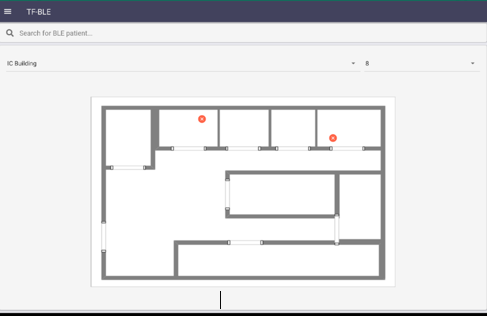
\includegraphics[width=\textwidth]{Image/bright1.png}
\caption{}
\label{bright1}
\end{figure}

\newpage
\paragraph{}In additional, it can track a wanted patient by press a search bar from Figure \ref{bright1} and then it will show the list of patients in Figure \ref{bright2}. Admin can input the word to filter the list and select patient and then it will display in Figure \ref{bright3}

\begin{figure}[h]
\centering
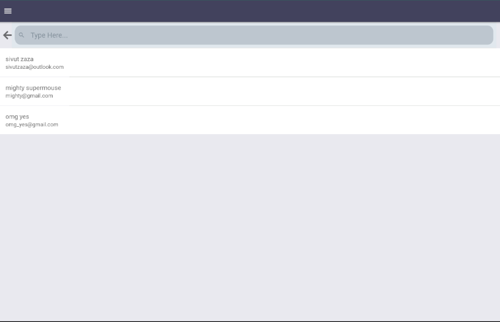
\includegraphics[width=\textwidth]{Image/bright2.png}
\caption{}
\label{bright2}
\end{figure}

\begin{figure}[h]
\centering
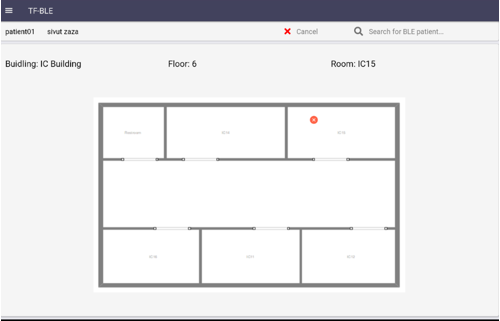
\includegraphics[width=\textwidth]{Image/bright3.png}
\caption{}
\label{bright3}
\end{figure}

\newpage
\newpage
In outdoor position tracking page, it works same as an indoor position page. It displays all patients that already outside the hospital area. Below are some of the user interface of the outdoor position tracking page as Figure \ref{bright4} . Moreover, it can track wanted patient by press a search bar in Figure \ref{bright4} and then it will show the lists of outside patients same as indoor positioning mode in Figure \ref{bright2}. After select wanted patient, it will display in Figure \ref{bright5}     
    

\begin{figure}[h]
\centering
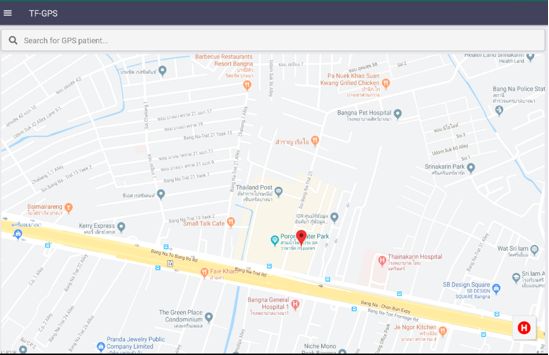
\includegraphics[width=\textwidth]{Image/bright4.png}
\caption{}
\label{bright4}
\end{figure}



\begin{figure}[h]
\centering
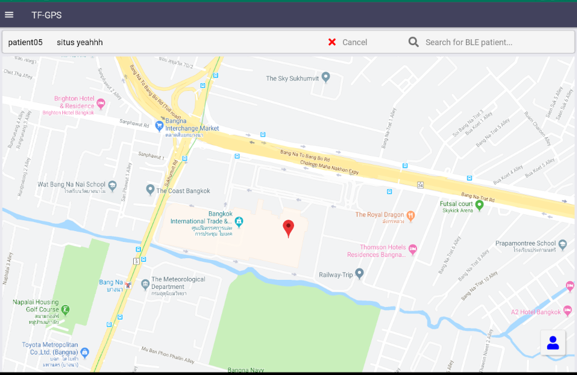
\includegraphics[width=\textwidth]{Image/bright5.png}
\caption{}
\label{bright5}
\end{figure}

